\section{Introduction}
Recent advancements in Large Language Models~(LLMs) have demonstrated outstanding proficiency in a wide range of text generation scenarios, such as content creation, abstractive text summarization, and instruction-following~\cite{thoppilan2022lamda,wei2022emergent,wang-etal-2023-self-instruct,llama,llama2}. Nevertheless, deploying LLMs is a notably costly undertaking considering their tremendous parameter size and quadratic cost of attention layers. Accordingly, model compression~\cite{frantar2023massive,xia2023sheared} and memory-efficient attention~\cite{dao2022flashattention,dao2023flashattention} techniques have emerged to tackle these challenges and achieved substantial outcomes.

\begin{figure}[t]
    \centering
    \scalebox{0.5}{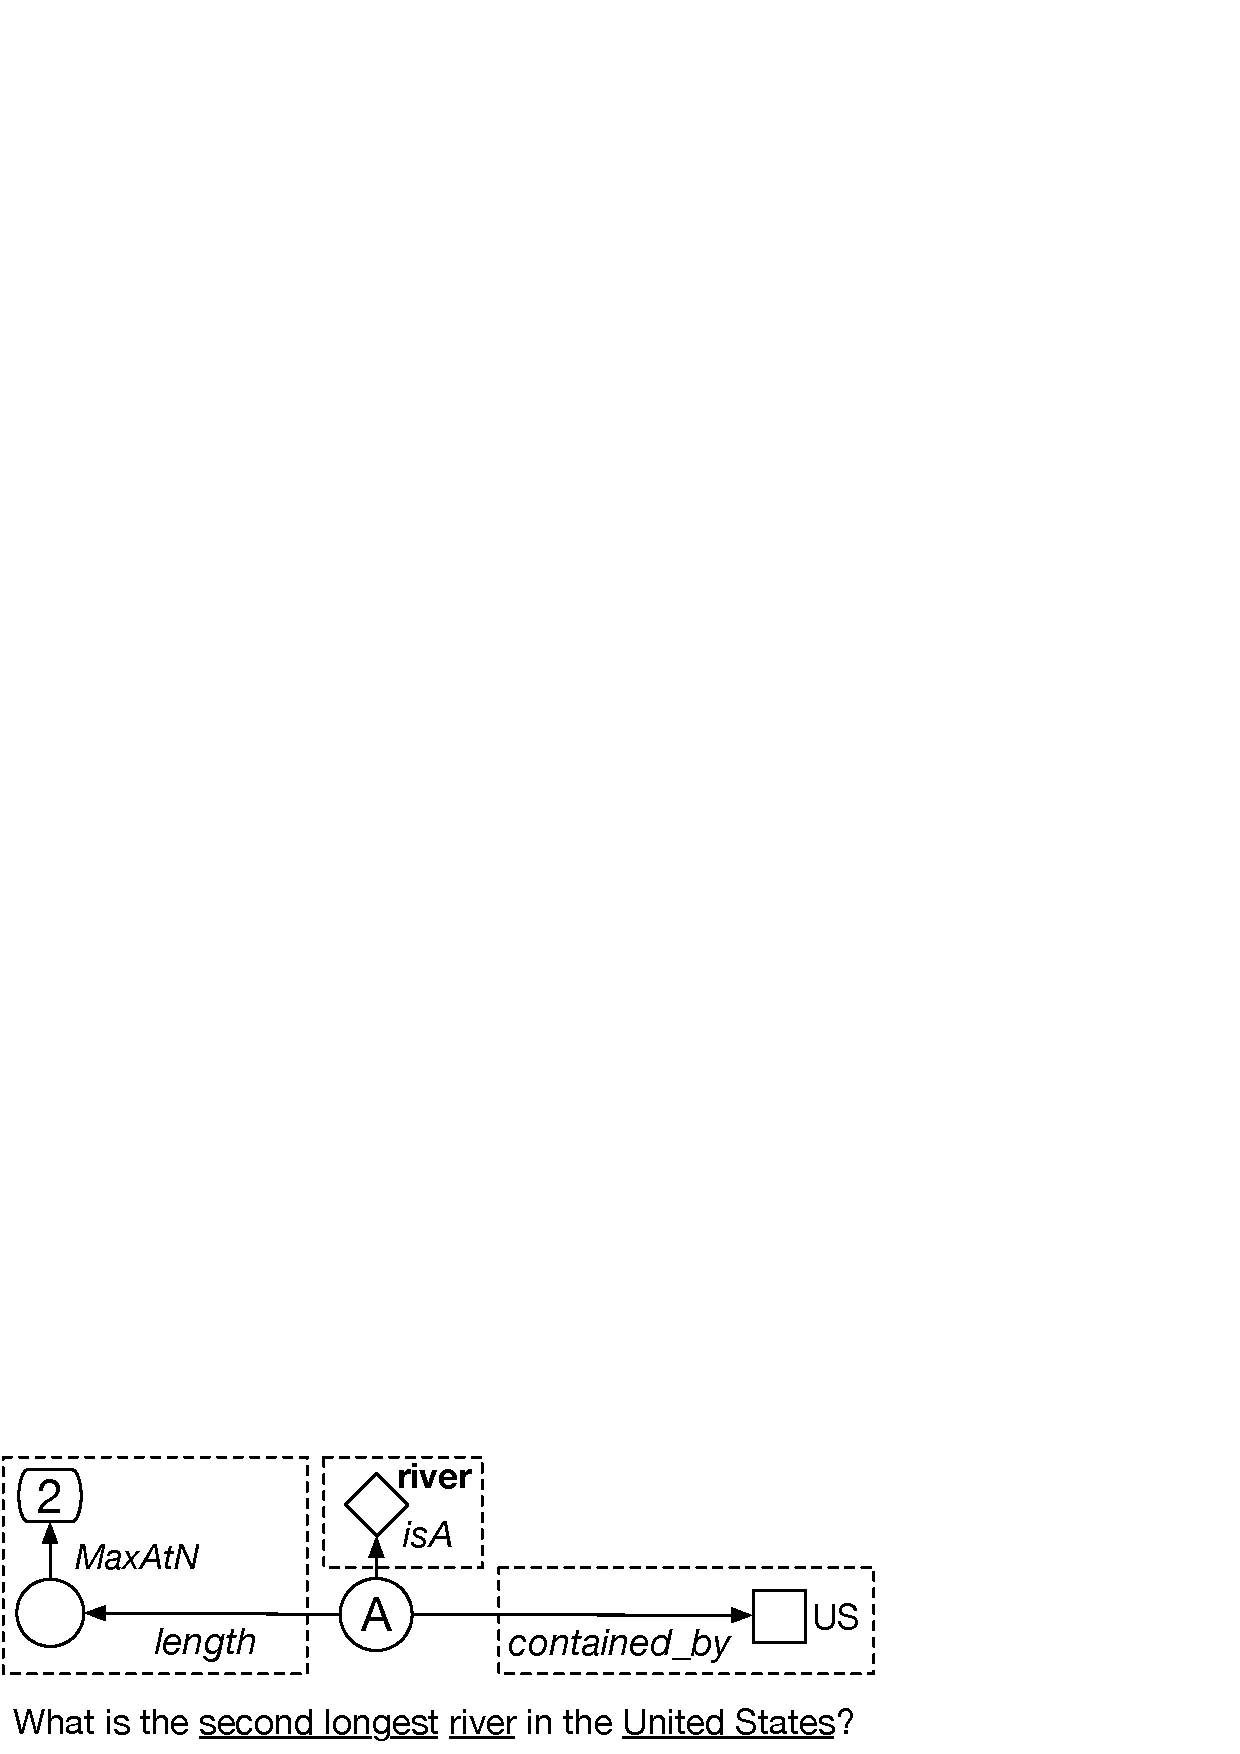
\includegraphics{./figures/intro.pdf}}
    \caption{Illustration of KV cache eviction inside one attention layer~($L$ in total). In this example, a single pair of key-value vectors are deleted~(red hatched areas) before appending the next token's. Different heads~($H$ in total) at model layers may evict at different positions.}
	\label{fig:intro}
\end{figure}
Owning to the auto-regressive nature of LLM inference~\cite{vaswani2017attention,radford2019language}, the intermediate attention key-value vectors are also required to be stored in memory to avoid redundant key-value projection in future steps. The size of key-value cache~(KV cache) depends on the configuration of the attention layer, batch size, and sequence length, which poses challenges in both memory footprint, I/O cost, and computation burden given the increasingly upsoaring model scale and user requests. Variants like multi-query attention and grouped-query attention~\cite{mqa,gqa} reduce the size of the KV cache with fewer attention heads, but cannot be directly applied to pre-trained LLMs without re-training. 

In pursuit of flexible and training-free control over KV cache during LLM inference, recent works~\cite{liu2023scissorhands,h2o,xiao2023efficient,tova} have investigated implementing KV cache with \textit{eviction policy}, where the key-value vectors of certain tokens are strategically deleted from memory~(see \figref{fig:intro}). In this way, the size of the KV cache can be maintained under a specified budget, leading to decreased memory and computational overhead. Despite the claimed and empirically observed reduction in KV cache, there still lacks a comprehensive comparative analysis of these methods. This study aims to fill this gap and embarks on the efficacy of existing eviction policies from a unified framework, which decomposes an eviction policy into two design dimensions: \textit{importance score calculation} and \textit{eviction scope construction}. 
The former characterizes how important a pair of key-value vectors is to future generations, 
while the latter determines which tokens are readily allowed to be evicted from the cache
We categorize existing eviction policies according to these two dimensions. 
Following our preliminary analysis, we discover that the way current methods calculate 
importance scores utilizing local statistics can only weakly approximate that derived 
from global statistics~(full KV cache without eviction). 
Moreover, prior methods commonly 
construct the eviction scope by only incorporating tokens outside of a local window, 
which we show endure high sensitivity to window size. 

In this paper, we propose RoCo, a \underline{R}\underline{o}bust \underline{C}ache \underline{o}mission policy based on local attention scores and robustness measures. Specifically, we compute the importance score of each in-cache token using averaged attention probability from future tokens, 
and formulate the eviction scope using tokens with the lowest variance of attention. 
RoCo exhibits significantly better consistency with 
full KV cache counterpart and robustness to eviction scope size.

To evaluate the effectiveness of RoCo in terms 
of preserving the LLM's downstream performance, we perform experiments across 
both prefilling and auto-regressive decoding stages at which cache eviction happens, 
spanning tasks of language modeling, text summarization, context reconstruction, and 
instruction following. Experimental results at different levels of KV cache 
budget demonstrates that RoCo results in significantly better generation 
quality compared to current methods judged by both automatic metrics and LLM-based evaluator.

Our contributions are summarized as follows:
\begin{itemize}[itemsep=1pt,parsep=2pt,topsep=1pt]
    \item We systematically analyze current cache eviction policies from the dimensions of importance score calculation and eviction scope construction, shedding light on their limitations.
    \item Based on our analysis, we introduce a robust cache omission policy named RoCo and conduct a comprehensive evaluation to verify its effectiveness on downstream tasks.
    \item We open-source EasyKV, a versatile software package that supports key-value constrained generative LLM inference with flexible configuration on cache budget and eviction policy.
\end{itemize}